% ============================================================================
% Control de formaciones en AttaBot
%
% Compilar con:  pdflatex formaciones.tex   (dos veces, por las referencias)
% Requiere: babel, amsmath, amssymb, amsthm, tikz, booktabs, algorithm,
%           algpseudocode, geometry, hyperref  — todo de una TeX Live estandar.
% ============================================================================

\documentclass[11pt,a4paper]{article}

\usepackage[T1]{fontenc}
\usepackage[utf8]{inputenc}
% Hay dos mecanismos de espanol en babel y no aceptan la misma sintaxis:
%   - el clasico spanish.ldf (CTAN babel-spanish, texlive-langspanish en Arch),
%     que es el que espera \usepackage[spanish]{babel};
%   - el nuevo basado en babel-es.ini, que viene con babel core y con el que
%     esa misma linea falla con "Unknown option 'spanish'".
% Se detecta cual hay para que el documento compile en las dos.
\IfFileExists{spanish.ldf}{%
  \usepackage[spanish]{babel}%
}{%
  \usepackage{babel}%
  \babelprovide[import,main]{spanish}%
}
\usepackage[margin=2.6cm]{geometry}

\usepackage{amsmath,amssymb,amsthm}
\usepackage{booktabs}
\usepackage{float}
\usepackage{algorithm}
\usepackage{algpseudocode}
\usepackage{tikz}
\usetikzlibrary{arrows.meta,positioning,calc}

% ---------------------------------------------------------------- colores ---
% xcolor ANTES que hyperref: las opciones de color de hyperref se evaluan al
% cargarlo, asi que los \definecolor tienen que existir ya.
\usepackage{xcolor}
\definecolor{colsteel}{HTML}{1F6273}
\definecolor{colamber}{HTML}{96660C}
\definecolor{colwrong}{HTML}{96371F}

\usepackage[colorlinks=true,linkcolor=colsteel,citecolor=colsteel,
            urlcolor=colsteel]{hyperref}

% \renewcommand a secas no alcanza: babel reinstala sus nombres al empezar el
% documento, asi que esto va despues.
\AtBeginDocument{\renewcommand{\tablename}{Tabla}}

% ------------------------------------------------------------- teoremas -----
\theoremstyle{plain}
\newtheorem{proposicion}{Proposición}
\renewcommand{\proofname}{Demostración}

% --------------------------------------------------- pseudocodigo en es -----
\floatname{algorithm}{Algoritmo}
\algrenewcommand\algorithmicif{\textbf{si}}
\algrenewcommand\algorithmicthen{\textbf{entonces}}
\algrenewcommand\algorithmicelse{\textbf{si no}}
\algrenewcommand\algorithmicend{\textbf{fin}}
\algrenewcommand\algorithmicfor{\textbf{para}}
\algrenewcommand\algorithmicforall{\textbf{para cada}}
\algrenewcommand\algorithmicdo{\textbf{hacer}}
\algrenewcommand\algorithmicwhile{\textbf{mientras}}
\algrenewcommand\algorithmicreturn{\textbf{devolver}}
\algrenewcommand\algorithmicprocedure{\textbf{procedimiento}}
\algrenewcommand\algorithmicrequire{\textbf{Entrada:}}
\algrenewcommand\algorithmicensure{\textbf{Salida:}}

% ------------------------------------------------------------- atajos -------
\newcommand{\cmd}[1]{\texttt{#1}}
\newcommand{\hh}{\hat{h}}
\newcommand{\pp}{\hat{p}}
\newcommand{\aaa}{\hat{a}}
\newcommand{\cruce}[2]{%
  \draw[colwrong,line width=1.1pt] ({#1-0.12},{#2-0.12}) -- ({#1+0.12},{#2+0.12});
  \draw[colwrong,line width=1.1pt] ({#1-0.12},{#2+0.12}) -- ({#1+0.12},{#2-0.12});}

\title{\bfseries Control de formaciones en AttaBot}
\author{Eduardo Fallas Valverde}
\date{13 de agosto de 2026}

\begin{document}
\maketitle

\begin{abstract}
\noindent
Cómo un grupo de robots diferenciales se acomoda en línea, cuña o círculo
alrededor de un líder móvil: qué decide la estación base, qué difunde el líder
y qué calcula cada seguidor por su cuenta. Se documentan las ecuaciones tal
como corren en el firmware, se demuestra que el reparto de posiciones no
produce cruces de trayectoria, y se describe un error de escala de factor
$\sqrt{2}$ que la figura en cuña arrastró hasta ser medido en laboratorio el
13 de agosto de 2026. Ambas figuras quedaron validadas en hardware con cuatro
robots: la línea con un error de 7\,mm en el slot más lejano, y la cuña
corregida con 23 a 37\,mm, después de que la misma medición mostrara el factor
$1{,}41$ desapareciendo entre una corrida y la siguiente.
\end{abstract}

\tableofcontents
\bigskip

% ============================================================================
\section{El reparto de trabajo}
% ============================================================================

Una formación se podría resolver entera en la estación base: ella ve a todos
los robots por la cámara cenital, podría calcular cada destino y transmitirlo.
No se hace así, y la razón es que el líder \emph{se mueve}. Si la base tuviera
que recalcular y retransmitir cuatro destinos cada vez que el líder avanza un
centímetro, la formación viviría al ritmo del enlace inalámbrico y se rompería
con cada paquete perdido.

En vez de eso el trabajo se parte en tres, según qué información hace falta
para cada decisión:

\begin{itemize}
  \item \textbf{Qué slot le toca a cada robot} lo decide la base, \emph{una
    sola vez}. Es la única que ve a todos a la vez, y sin esa vista global no
    se puede evitar que dos robots crucen trayectorias.
  \item \textbf{Dónde está el marco de referencia} lo difunde el líder,
    continuamente. La formación se define respecto de \emph{él}, no de la
    arena.
  \item \textbf{Dónde queda mi slot y cómo llego} lo calcula cada seguidor,
    localmente, cada vez que le llega una pose del líder.
\end{itemize}

El resultado es que si la base se cae después de repartir los índices, la
formación sigue viva: los seguidores tienen todo lo que necesitan mientras el
líder siga difundiendo. Ese es el grado intermedio de centralización de la
plataforma, entre el comando central robot por robot y la coordinación
puramente local.

\begin{figure}[H]
\centering
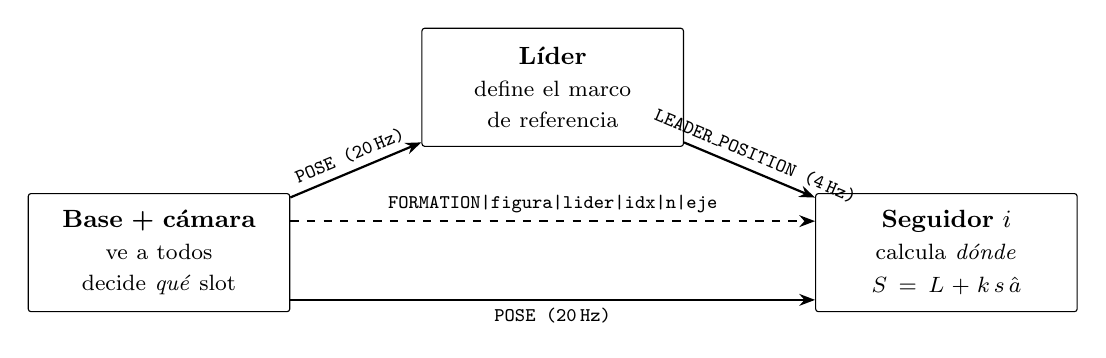
\begin{tikzpicture}[
  font=\small,
  box/.style={draw,rounded corners=1pt,align=center,inner sep=6pt,
              text width=2.9cm,minimum height=1.5cm},
  flow/.style={-{Stealth[length=2mm]},thick},
  lbl/.style={font=\scriptsize\ttfamily,inner sep=2.5pt},
]
  \node[box] (base)  at (0,0)     {\textbf{Base + cámara}\\[2pt]
                                   \footnotesize ve a todos\\
                                   \footnotesize decide \emph{qué} slot};
  \node[box] (lider) at (5.0,2.1) {\textbf{Líder}\\[2pt]
                                   \footnotesize define el marco\\
                                   \footnotesize de referencia};
  \node[box] (seg)   at (10.0,0)  {\textbf{Seguidor $i$}\\[2pt]
                                   \footnotesize calcula \emph{dónde}\\[1pt]
                                   $S = L + k\,s\,\aaa$};

  \draw[flow] (base) -- node[lbl,sloped,above] {POSE (20\,Hz)} (lider);
  \draw[flow] (lider) -- node[lbl,sloped,above] {LEADER\_POSITION (4\,Hz)} (seg);

  \draw[flow,dashed] ([yshift=4mm]base.east) --
        node[lbl,above] {FORMATION|figura|lider|idx|n|eje}
        ([yshift=4mm]seg.west);
  \draw[flow] ([yshift=-6mm]base.east) --
        node[lbl,below] {POSE (20\,Hz)} ([yshift=-6mm]seg.west);
\end{tikzpicture}
\caption{El índice de slot viaja una sola vez (línea punteada); todo lo demás
es un lazo continuo. La pose del líder va por difusión, de modo que un seguidor
más no cuesta un mensaje más. Cortar la punteada después del arranque no rompe
la formación; cortar la del líder sí.}
\label{fig:pipeline}
\end{figure}

\subsection*{Notación}

\noindent
\begin{tabular}{@{}ll@{}}
  $L$, $\theta_L$ & posición y rumbo del líder \\
  $s$             & espaciado pedido, en mm (\cmd{NAV\_CONFIG|PARKING\_DIST}) \\
  $n$             & cantidad de seguidores \\
  $i$             & índice de slot del seguidor, $0 \le i < n$ \\
  $\alpha$        & giro opcional del eje de la fila \\
  $\hh$, $\pp$    & versores del rumbo del líder y del eje de la fila \\
  $\aaa$          & versor del brazo sobre el que se reparten los slots \\
  $S_i$           & posición del slot $i$ \\
  $W_i$           & waypoint de aproximación (\emph{staging}) del slot $i$ \\
\end{tabular}

% ============================================================================
\section{Etapa 1: la base reparte los slots}
% ============================================================================

El problema no es dónde poner los robots, que lo fija la figura, sino
\emph{cuál va en cuál}. Con tres seguidores hay seis asignaciones posibles y
cinco de ellas hacen que al menos dos robots se crucen de camino. Cruzarse en
una arena de $2{,}4 \times 1{,}75$\,m con navegación reactiva significa que se
detectan mutuamente como obstáculo, se evaden, y la formación tarda el doble o
entra en bloqueo.

La solución es un emparejamiento monótono. Se proyecta cada seguidor sobre el
eje de la fila, se ordenan los slots sobre ese mismo eje, y se emparejan por
rango: el que ya está más a la izquierda recibe el slot más a la izquierda.

\begin{align}
  \pp &= \bigl(\cos(\theta_L + 90^\circ + \alpha),\;
               \sin(\theta_L + 90^\circ + \alpha)\bigr)
  \label{eq:eje}\\[2pt]
  \kappa(j) &= (P_j - L)\cdot\pp
  \label{eq:clave-seg}\\[2pt]
  \kappa_s(i) &= \sigma(i)\,k(i)
  \label{eq:clave-slot}
\end{align}

\noindent
donde $P_j$ es la posición del seguidor $j$, y $k(i)$ y $\sigma(i)$ son el
anillo y el lado que se definen en la ecuación~\eqref{eq:anillo}. Para la
figura en círculo las claves son angulares:
$\kappa(j) = \operatorname{atan2}(y_j - y_L,\, x_j - x_L) \bmod 2\pi$ y
$\kappa_s(i) = 2\pi i / n$.

Ambas listas se ordenan de menor a mayor y se emparejan por posición en el
orden.

% ----------------------------------------------------------------------------
\subsection{Por qué el orden por rango no cruza}
% ----------------------------------------------------------------------------

\begin{proposicion}\label{prop:cruces}
Sean $a_1 \le a_2 \le \dots \le a_n$ las coordenadas de los seguidores sobre el
eje $\pp$ y $b_1 < b_2 < \dots < b_n$ las de los slots sobre ese mismo eje. Si
cada seguidor $i$ se dirige al slot $i$ recorriendo un segmento recto, entonces
para todo par $i < j$ y todo instante normalizado $t \in [0,1)$ se cumple
$p_j(t) > p_i(t)$; en particular, dos robots nunca ocupan el mismo punto del
plano.
\end{proposicion}

\begin{proof}
La coordenada proyectada del robot $i$ en el instante $t$ es la interpolación
\begin{equation}
  p_i(t) = (1-t)\,a_i + t\,b_i, \qquad t\in[0,1].
  \label{eq:trayectoria}
\end{equation}
Restando dos de ellas,
\begin{equation}
  p_j(t) - p_i(t) = (1-t)\,(a_j - a_i) \;+\; t\,(b_j - b_i).
  \label{eq:separacion}
\end{equation}
Por construcción del emparejamiento por rango, $j > i$ implica $a_j \ge a_i$ y
$b_j > b_i$, de modo que ambos sumandos de~\eqref{eq:separacion} son no
negativos y el segundo es estrictamente positivo para $t > 0$. Una combinación
convexa de cantidades no negativas no cambia de signo, luego
$p_j(t) - p_i(t) > 0$ en todo el recorrido. Dos puntos del plano con distinta
proyección sobre $\pp$ son distintos, así que no hay cruce ni colisión.
\end{proof}

El recíproco cae solo y explica por qué cualquier otra asignación falla:
un emparejamiento distinto introduce al menos una inversión, es decir un par
con $a_i < a_j$ pero $b_i > b_j$. Ahí los dos sumandos
de~\eqref{eq:separacion} tienen signos opuestos, la diferencia es continua y
cambia de signo, y por el teorema del valor intermedio se anula en algún $t$
interior. Ese cero \emph{es} el cruce.

\begin{figure}[H]
\centering
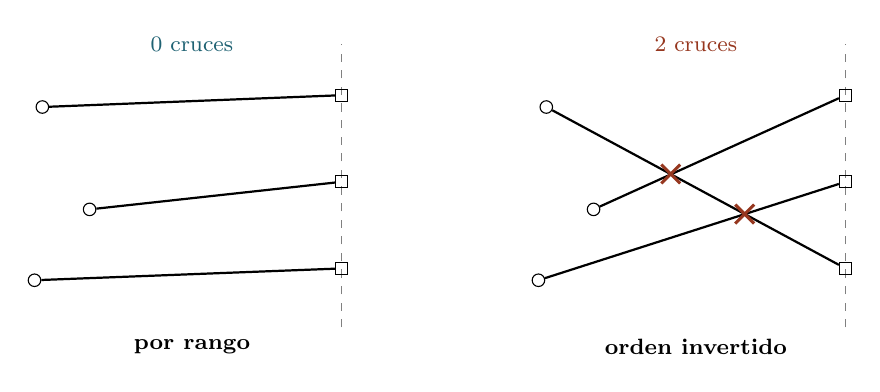
\begin{tikzpicture}[
  font=\small,
  seg/.style={draw,circle,inner sep=1.6pt},
  slot/.style={draw,rectangle,inner sep=2.2pt},
  path/.style={thick},
]
  % ---- panel izquierdo: por rango ----
  \begin{scope}
    \draw[dashed,gray] (3.8,-1.7) -- (3.8,1.9);
    \node[seg]  (a1) at (0,1.1)   {};
    \node[seg]  (a2) at (0.6,-0.2){};
    \node[seg]  (a3) at (-0.1,-1.1){};
    \node[slot] (b1) at (3.8,1.25) {};
    \node[slot] (b2) at (3.8,0.15) {};
    \node[slot] (b3) at (3.8,-0.95){};
    \draw[path] (a1) -- (b1);
    \draw[path] (a2) -- (b2);
    \draw[path] (a3) -- (b3);
    \node[font=\footnotesize] at (1.9,-1.95) {\textbf{por rango}};
    \node[font=\footnotesize,colsteel] at (1.9,1.9) {0 cruces};
  \end{scope}
  % ---- panel derecho: orden invertido ----
  \begin{scope}[xshift=6.4cm]
    \draw[dashed,gray] (3.8,-1.7) -- (3.8,1.9);
    \node[seg]  (c1) at (0,1.1)    {};
    \node[seg]  (c2) at (0.6,-0.2) {};
    \node[seg]  (c3) at (-0.1,-1.1){};
    \node[slot] (d1) at (3.8,1.25) {};
    \node[slot] (d2) at (3.8,0.15) {};
    \node[slot] (d3) at (3.8,-0.95){};
    \draw[path] (c1) -- (d3);
    \draw[path] (c2) -- (d1);
    \draw[path] (c3) -- (d2);
    \cruce{1.58}{0.25}
    \cruce{2.52}{-0.26}
    \node[font=\footnotesize] at (1.9,-1.95) {\textbf{orden invertido}};
    \node[font=\footnotesize,colwrong] at (1.9,1.9) {2 cruces};
  \end{scope}
\end{tikzpicture}
\caption{Círculos: dónde está cada seguidor. Cuadrados: los slots sobre el eje
de la fila. Emparejar por rango conserva el orden y las trayectorias quedan
paralelas; una sola inversión basta para producir cruces, y cada cruce es una
evasión mutua en la arena real.}
\label{fig:cruces}
\end{figure}

% ----------------------------------------------------------------------------
\subsection{Qué no garantiza}
% ----------------------------------------------------------------------------

La proposición~\ref{prop:cruces} es limpia pero angosta, y vale más saber dónde
termina:

\begin{itemize}
  \item \textbf{Es sobre la geometría planificada, no sobre la trayectoria
    ejecutada.} Los robots no van en línea recta: pasan por un waypoint de
    aproximación, avanzan a velocidades distintas y desvían por evasión
    reactiva. La garantía dice que los \emph{destinos} no obligan a cruzarse,
    no que el recorrido real no lo haga.
  \item \textbf{Es topológica, no métrica.} Conserva el orden, no la
    separación. Dos robots pueden mantener el orden y aun así acercarse lo
    suficiente para dispararse la evasión por infrarrojo.
  \item \textbf{Supone el líder quieto durante el tránsito.} Si se mueve, los
    slots se mueven con él y las $b_i$ dejan de ser constantes.
  \item \textbf{Los robots que la cámara no ve quedan fuera del argumento.}
    Reciben $\kappa = +\infty$ y el slot que sobra, de modo que su posición
    real no participa del orden. La base lo advierte explícitamente cuando
    ocurre. Conviene notar que devolver $0$ en lugar de $+\infty$ ---como se
    hacía antes--- es peor que no ordenar: $0$ es una coordenada lateral
    perfectamente válida, así que un robot invisible se colaba entre los
    visibles y les corría el slot a todos, degradando la asignación en
    silencio justo cuando más falta hacía.
  \item \textbf{La figura en círculo no hereda la garantía.} Sobre una
    circunferencia el orden es cíclico y el corte en $0^\circ$ es arbitrario.
    El emparejamiento sin cruces en un ciclo exige elegir el desplazamiento
    rotacional correcto entre $n$ posibles; ordenar por rango con un corte fijo
    es sólo uno de esos $n$, y no siempre el bueno. Para el círculo la
    asignación es una heurística razonable, no un teorema.
\end{itemize}

% ----------------------------------------------------------------------------
\subsection{Validación contra la arena}
% ----------------------------------------------------------------------------

Antes de transmitir nada, la base comprueba que todo slot caiga dentro de la
arena con un margen de 250\,mm respecto de las paredes. Si una fila
perpendicular no cabe, se reintenta con el eje girado $\alpha = 90^\circ$
---la fila se vuelve columna--- antes de rechazar. Si aun así no cabe, el
mensaje de error indica qué slot falla y por cuántos milímetros: un rechazo por
9\,mm y uno por medio metro exigen acciones distintas del operador.

El círculo es la excepción y no se valida aquí, porque el firmware lo resuelve
con su propio algoritmo de anillo seguro (sección~\ref{sec:anillo}) y
compararlo contra un anillo plano de radio nominal sólo producía rechazos
falsos.

% ============================================================================
\section{Etapa 2: el líder difunde su pose}
% ============================================================================

El líder recibe su propia pose de la base a unos 20\,Hz y la reemite por
difusión, pero limitada a 4\,Hz. Reemitir las veinte saturaría el enlace sin
aportar nada, porque los seguidores no replanifican más rápido que eso.

Antes de difundir, la pose pasa por una media móvil de $N = 4$ muestras. El
ángulo no se puede promediar directamente ---entre $359^\circ$ y $1^\circ$ el
promedio aritmético da $180^\circ$, exactamente el lado contrario--- así que se
promedian el seno y el coseno y se recompone:

\begin{align}
  \bar{x} &= \frac{1}{N}\sum_t x_t,
  \qquad
  \bar{y} = \frac{1}{N}\sum_t y_t
  \label{eq:media-pos}\\[2pt]
  \bar{\theta} &= \operatorname{atan2}
     \Bigl(\textstyle\sum_t \sin\theta_t,\; \sum_t \cos\theta_t\Bigr)
  \label{eq:media-ang}
\end{align}

La ventana se vacía si la muestra nueva cae a más de 100\,mm de la media
vigente: en ese caso el líder se movió de verdad, o la cámara lo leyó mal, y en
cualquiera de los dos casos promediar con lo viejo introduce un retardo que
miente.

Del lado del seguidor hay una segunda defensa contra el ruido: el objetivo de
navegación sólo se reubica si el nuevo cae a más de 40\,mm del actual. Sin esa
banda muerta el destino se corría unos milímetros con cada mensaje y el
navegador terminaba re-apuntando contra el ruido de la localización visual en
vez de contra el movimiento real del líder.

% ============================================================================
\section{Etapa 3: el seguidor calcula su slot}
% ============================================================================

Cada seguidor conoce cuatro cosas: la pose del líder que acaba de llegar, su
índice $i$, el total $n$ y el espaciado $s$. Con eso arma la posición de su
slot sin hablar con nadie.

El índice se descompone en \emph{anillo} y \emph{lado}: los pares van a un
lado, los impares al otro, y cada par de índices sube un anillo.

\begin{equation}
  k(i) = \left\lfloor i/2 \right\rfloor + 1,
  \qquad
  \sigma(i) = \begin{cases} +1 & i \text{ par}\\ -1 & i \text{ impar}\end{cases}
  \label{eq:anillo}
\end{equation}

Con $\hh = (\cos\theta_L, \sin\theta_L)$ el versor del rumbo del líder y $\pp$
el de la ecuación~\eqref{eq:eje}, la dirección del brazo y la posición del slot
son

\begin{align}
  \aaa(i) &= \begin{cases}
      \sigma(i)\,\pp & \text{línea}\\[4pt]
      \dfrac{\sigma(i)\,\pp - \hh}{\sqrt{2}} & \text{cuña}
    \end{cases}
  \label{eq:brazo}\\[6pt]
  S_i &= L + k(i)\,s\,\aaa(i)
  \label{eq:slot}
\end{align}

La normalización de la cuña no es cosmética. Como $\pp$ y $\hh$ son unitarios y
perpendiculares, $\lVert \sigma\pp - \hh \rVert = \sqrt{2}$; dividir por
$\sqrt{2}$ es lo que hace que $s$ signifique lo mismo en las dos figuras:
distancia del líder al primer slot, y separación entre slots consecutivos del
mismo brazo. Que el brazo caiga exactamente a $135^\circ$ se sigue de ahí:

\begin{equation}
  \aaa\cdot\hh
  = \frac{\sigma\,(\pp\cdot\hh) - \hh\cdot\hh}{\sqrt{2}}
  = \frac{0 - 1}{\sqrt{2}}
  = -\frac{\sqrt{2}}{2}
  \quad\Longrightarrow\quad
  \angle(\aaa,\hh) = 135^\circ .
  \label{eq:135}
\end{equation}

\begin{figure}[H]
\centering
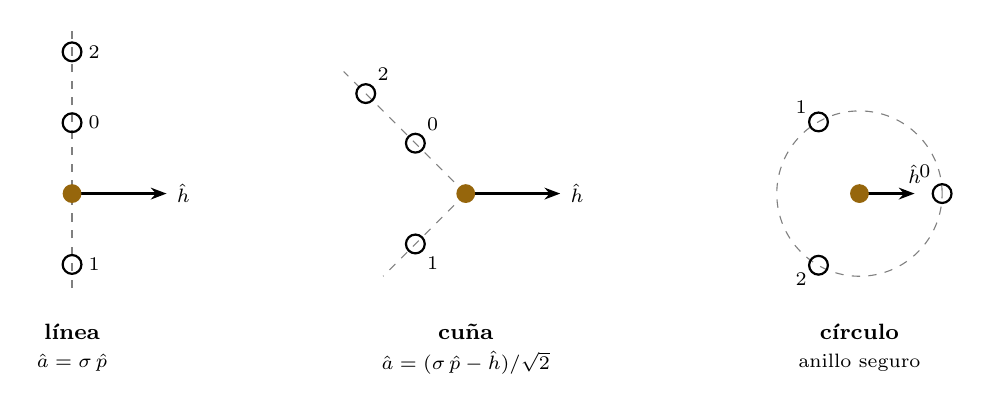
\begin{tikzpicture}[
  font=\small,
  lead/.style={circle,fill=colamber,inner sep=2.4pt},
  slot/.style={circle,draw,thick,inner sep=2.4pt},
  ray/.style={dashed,gray},
  head/.style={-{Stealth[length=2mm]},thick},
]
  % ---------------- linea ----------------
  \begin{scope}
    \draw[ray] (0,-1.2) -- (0,2.1);
    \draw[head] (0,0) -- (1.2,0) node[right,font=\scriptsize] {$\hh$};
    \node[lead] at (0,0) {};
    \node[slot] at (0,0.9)  {}; \node[font=\scriptsize] at (0.28,0.9)  {0};
    \node[slot] at (0,-0.9) {}; \node[font=\scriptsize] at (0.28,-0.9) {1};
    \node[slot] at (0,1.8)  {}; \node[font=\scriptsize] at (0.28,1.8)  {2};
    \node[font=\footnotesize] at (0,-1.75) {\textbf{línea}};
    \node[font=\scriptsize]   at (0,-2.15) {$\aaa = \sigma\,\pp$};
  \end{scope}
  % ---------------- cuna ----------------
  \begin{scope}[xshift=5cm]
    \draw[ray] (0,0) -- (-1.55,1.55);
    \draw[ray] (0,0) -- (-1.05,-1.05);
    \draw[head] (0,0) -- (1.2,0) node[right,font=\scriptsize] {$\hh$};
    \node[lead] at (0,0) {};
    \node[slot] at (-0.64,0.64)  {}; \node[font=\scriptsize] at (-0.42,0.88)  {0};
    \node[slot] at (-0.64,-0.64) {}; \node[font=\scriptsize] at (-0.42,-0.88) {1};
    \node[slot] at (-1.27,1.27)  {}; \node[font=\scriptsize] at (-1.05,1.51)  {2};
    \node[font=\footnotesize] at (0,-1.75) {\textbf{cuña}};
    \node[font=\scriptsize]   at (0,-2.15) {$\aaa = (\sigma\,\pp - \hh)/\sqrt{2}$};
  \end{scope}
  % ---------------- circulo ----------------
  \begin{scope}[xshift=10cm]
    \draw[ray] (0,0) circle (1.05);
    % flecha corta y etiqueta arriba: el slot 0 vive en (1.05,0) y con la
    % flecha larga se le montaba encima.
    \draw[head] (0,0) -- (0.7,0) node[above,font=\scriptsize] {$\hh$};
    \node[lead] at (0,0) {};
    \node[slot] at (1.05,0)      {}; \node[font=\scriptsize] at (0.83,0.28)  {0};
    \node[slot] at (-0.52,0.91)  {}; \node[font=\scriptsize] at (-0.74,1.09) {1};
    \node[slot] at (-0.52,-0.91) {}; \node[font=\scriptsize] at (-0.74,-1.09){2};
    \node[font=\footnotesize] at (0,-1.75) {\textbf{círculo}};
    \node[font=\scriptsize]   at (0,-2.15) {anillo seguro};
  \end{scope}
\end{tikzpicture}
\caption{Vista en planta con el líder (punto lleno) y el rumbo hacia la
derecha. Los números son índices de slot: pares a un lado, impares al otro,
subiendo de anillo cada dos.}
\label{fig:figuras}
\end{figure}

% ----------------------------------------------------------------------------
\subsection{El anillo seguro del círculo}
\label{sec:anillo}
% ----------------------------------------------------------------------------

Un anillo de radio fijo alrededor de un líder pegado a la pared pone la mitad
de los slots fuera de la arena. En vez de rechazar la formación, el firmware
busca un anillo que sí entre: prueba radios crecientes
$g \in \{1,\; 1{,}2,\; 1{,}4,\; 1{,}7,\; 2{,}0,\; 2{,}5\}$, muestrea cada uno
en 72 puntos, y se queda con el arco contiguo más largo que respeta 200\,mm de
margen. Acepta ese radio si el arco alcanza para todos:

\begin{equation}
  R \cdot \text{arco} \;\ge\; n \cdot 250\,\text{mm},
  \qquad
  \varphi_i = a_0 + \Bigl(i + \tfrac{1}{2}\Bigr)\frac{\text{arco}}{n}
  \label{eq:anillo-seguro}
\end{equation}

Los 250\,mm por robot son el espacio mínimo para que no se toquen. Si ningún
radio cumple, se usa el mayor y se aprieta: mejor una formación apretada que
ninguna.

% ============================================================================
\section{Etapa 4: la entrada por aproximación}
% ============================================================================

Conocer el slot no basta: la recta desde donde está el robot hasta su slot
puede pasar por encima del líder o cruzar el slot de un vecino. Por eso la
navegación es en dos tramos, y el punto intermedio depende de la figura:

\begin{equation}
  W_i = \begin{cases}
    S_i - 150\,\hh
      & \text{línea y cuña}\\[4pt]
    L + (R + 150)\,(\cos\varphi_i,\; \sin\varphi_i)
      & \text{círculo}
  \end{cases}
  \label{eq:staging}
\end{equation}

En línea y cuña el waypoint queda 150\,mm por detrás del slot, de modo que cada
robot entra por su propio carril, paralelo al de los demás. En círculo la
aproximación es radial: se entra desde afuera del anillo, nunca cruzándolo. Al
alcanzar $W_i$ el robot marca la etapa como cumplida y el objetivo pasa a ser
$S_i$. De ahí en más sigue recalculando el slot con cada difusión del líder, de
modo que si el líder se mueve la formación lo acompaña.

% ============================================================================
\section{El factor \texorpdfstring{$\sqrt{2}$}{raiz de 2} de la cuña}
% ============================================================================

La cuña estuvo mal desde que se escribió, y el error sobrevivió a la revisión
porque producía una figura que \emph{se ve bien}: simétrica, con los dos brazos
a $135^\circ$, los robots ordenados. Lo único incorrecto era la escala, y una
escala equivocada no se nota a ojo.

El código sumaba dos desplazamientos, cada uno de magnitud $k\,s$: uno lateral
y uno hacia atrás. Como son perpendiculares, la suma no mide $k\,s$ sino su
hipotenusa:

\begin{align}
  o_i^{\text{(antes)}} &= k\,s\,(\sigma\pp) - k\,s\,\hh
  &&\Longrightarrow&
  \lVert o_i \rVert &= k\,s\,\sqrt{2} \approx 1{,}414\,k\,s
  \label{eq:bug}\\[2pt]
  o_i^{\text{(ahora)}} &= k\,s\,\frac{\sigma\pp - \hh}{\sqrt{2}}
  &&\Longrightarrow&
  \lVert o_i \rVert &= k\,s
  \label{eq:fix}
\end{align}

\begin{figure}[H]
\centering
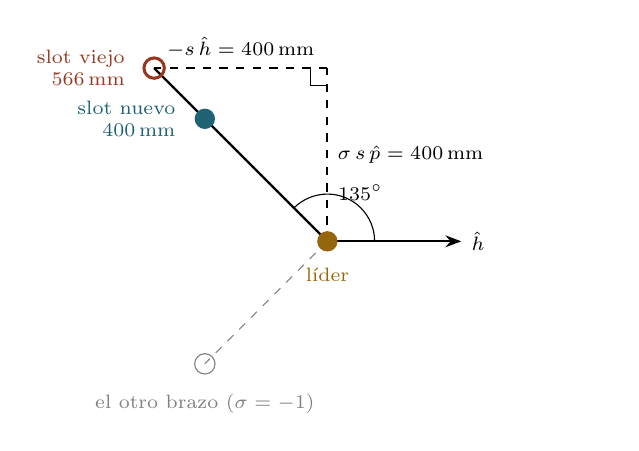
\begin{tikzpicture}[
  font=\small,
  head/.style={-{Stealth[length=2mm]},thick},
  leg/.style={dashed,thick},
]
  \coordinate (L) at (0,0);
  \coordinate (A) at (0,2.2);
  \coordinate (B) at (-2.2,2.2);
  \coordinate (C) at (-1.556,1.556);
  \coordinate (M) at (-1.556,-1.556);

  % Fuerza un cuadro simetrico: las etiquetas de la izquierda son largas y sin
  % esto el dibujo queda visiblemente corrido a la derecha de la caja.
  \path (-3.6,0) (3.6,0);

  % Sin rotulo "rumbo del lider": arriba de la flecha se le monta al arco de
  % 135 grados y abajo al nombre del lider. La tabla de notacion ya define h.
  \draw[head] (L) -- (1.7,0) node[right,font=\scriptsize] {$\hh$};

  \draw[leg] (L) -- (A) node[midway,right,font=\scriptsize]
        {$\sigma\,s\,\pp = 400$\,mm};
  \draw[leg] (A) -- (B) node[midway,above,font=\scriptsize]
        {$-s\,\hh = 400$\,mm};
  \draw (-0.22,2.2) -- (-0.22,1.98) -- (0,1.98);   % angulo recto

  \draw[thick] (L) -- (B);
  \draw[gray,dashed] (L) -- (M);

  \draw (0.6,0) arc[start angle=0, end angle=135, radius=0.6];
  \node[font=\scriptsize] at (0.42,0.62) {$135^\circ$};

  \node[circle,draw=colwrong,line width=1.1pt,inner sep=2.6pt] at (B) {};
  \node[font=\scriptsize,colwrong,align=right,anchor=east] at ($(B)+(-0.25,0)$)
        {slot viejo\\$566$\,mm};

  \node[circle,fill=colsteel,inner sep=2.6pt] at (C) {};
  \node[font=\scriptsize,colsteel,align=right,anchor=east] at ($(C)+(-0.25,0)$)
        {slot nuevo\\$400$\,mm};

  \node[circle,fill=colamber,inner sep=2.6pt] at (L) {};
  \node[font=\scriptsize,colamber,anchor=north] at ($(L)+(0,-0.22)$) {líder};

  \node[circle,draw=gray,inner sep=2.6pt] at (M) {};
  \node[font=\scriptsize,gray,anchor=north] at ($(M)+(0,-0.26)$)
        {el otro brazo ($\sigma = -1$)};
\end{tikzpicture}
\caption{Con un espaciado pedido de 400\,mm, el slot caía en el vértice de la
hipotenusa en vez de sobre el rayo a 400\,mm. El ángulo del brazo siempre
estuvo bien; sólo estaba mal el módulo.}
\label{fig:sqrt2}
\end{figure}

Medido en laboratorio con \cmd{FORMATION|cuna|1|400}, los tres seguidores
quedaron a 535, 560 y 1149\,mm del líder, contra los 400, 400 y 800 pedidos.
Las razones son $1{,}338$, $1{,}400$ y $1{,}436$, repartidas alrededor de
$\sqrt{2} = 1{,}4142$; lo que sobra y falta es la tolerancia de llegada de
50\,mm más el ruido de la localización visual.

\paragraph{La trampa de la fórmula duplicada.}
La geometría del slot está escrita \textbf{dos veces}: en el firmware, que la
usa para navegar, y en la base, que la replica para validar contra los límites
de la arena. Arreglar sólo el firmware habría dejado a la base calculando slots
$1{,}4$ veces más lejos, y por lo tanto rechazando formaciones que en realidad
caben. Cualquier cambio en la fórmula toca los dos archivos.

% ============================================================================
\section{Validación en hardware}
% ============================================================================

La formación en línea funcionó por primera vez el 13 de agosto de 2026, después
de corregir la validación contra la arena, el rechazo de círculos válidos y los
seguidores invisibles que se colaban al medio. Tres corridas con cuatro robots,
líder \cmd{Atta\_1}, espaciado $s = 300$\,mm.

\begin{table}[H]
\centering
\begin{tabular}{@{}lrrr@{}}
  \toprule
  Corrida & Slot $-300$ & Slot $+300$ & Slot $+600$ \\
  \midrule
  13-10 & 319\,mm / $-87^\circ$ & 311\,mm / $+86^\circ$
        & 605\,mm / $+91^\circ$ \\
  13-18 & 316\,mm / $-86^\circ$ & 294\,mm / $+89^\circ$
        & \textcolor{colwrong}{769\,mm / $+108^\circ$} \\
  13-20 & 313\,mm / $+91^\circ$ & 297\,mm / $-92^\circ$
        & \textcolor{colsteel}{593\,mm / $+91^\circ$} \\
  \bottomrule
\end{tabular}
\caption{Distancia y ángulo de cada seguidor respecto del líder al final de la
corrida. El ángulo se mide desde el rumbo del líder.}
\label{tab:validacion}
\end{table}

La mejor corrida cierra con 7\,mm de error en el slot más lejano y menos de
$2^\circ$ de desviación angular, sobre robots de tracción diferencial con
odometría corregida por cámara. El único fallo ---el slot lejano de la
corrida 13-18--- fue de un robot que seguía moviéndose cuando se cortó el
registro y que ese mismo día concentró 17 de los 21 episodios de navegación sin
realimentación visual: el problema es su marcador fiducial, no la lógica de
slots.

\subsection*{La cuña, antes y después}

La corrección de la escala se cargó por aire ese mismo día, entre dos corridas
de cuña separadas por veinticinco minutos. Eso deja la comparación más limpia
que se puede pedir: mismo líder, mismo espaciado de 400\,mm, misma arena, misma
luz, y como única diferencia el firmware.

\begin{table}[H]
\centering
\begin{tabular}{@{}lrrr@{}}
  \toprule
  Corrida & Slot $+135^\circ$ & Slot $-135^\circ$ & Slot $+135^\circ$ ($k = 2$) \\
  \midrule
  \multicolumn{4}{@{}l}{\emph{pedido}} \\
   & 400\,mm & 400\,mm & 800\,mm \\[2pt]
  13-22 (antes)
    & \textcolor{colwrong}{560\,mm} ($\times 1{,}400$)
    & \textcolor{colwrong}{535\,mm} ($\times 1{,}338$)
    & \textcolor{colwrong}{1149\,mm} ($\times 1{,}436$) \\
  13-47 (después)
    & \textcolor{colsteel}{423\,mm} ($+23$)
    & \textcolor{colsteel}{425\,mm} ($+25$)
    & \textcolor{colsteel}{837\,mm} ($+37$) \\
  \bottomrule
\end{tabular}
\caption{Distancia de cada seguidor al líder al cierre de la corrida, mediana
de los últimos 8\,s del registro de posiciones. Los ángulos estuvieron bien en
las dos, entre $\pm 131^\circ$ y $\pm 139^\circ$.}
\label{tab:cuna}
\end{table}

El $\times 1{,}41$ repartido por igual entre los tres slots es la firma del
$\sqrt{2}$: un error de escala multiplica, no desplaza. Después de la
corrección el residuo cae a 23--37\,mm, del mismo orden que el de la línea y
por debajo de la tolerancia de llegada de 50\,mm. La cuña queda validada.

% ============================================================================
\section{Pseudocódigo}
% ============================================================================

\begin{algorithm}[H]
\caption{Reparto de slots (estación base, una sola vez)}
\label{alg:base}
\begin{algorithmic}[1]
\Procedure{Formación}{figura, líder, $s$}
  \State $L, \theta_L \gets$ pose del líder
  \If{el líder no es visible} \State \textbf{abortar} \EndIf
  \State $F \gets$ todos los robots menos el líder; \quad $n \gets |F|$
  \State $\alpha \gets 0$
  \Statex
  \Comment{¿caben todos los slots en la arena, con 250\,mm de margen?}
  \If{figura $\ne$ círculo \textbf{y} algún slot se sale}
    \If{figura $=$ línea \textbf{y} con $\alpha = 90^\circ$ sí cabe}
      \State $\alpha \gets 90^\circ$
      \Comment{la fila se vuelve columna}
    \Else
      \State informar qué slot falla y por cuántos mm
      \State \textbf{abortar}
    \EndIf
  \EndIf
  \Statex
  \Comment{asignación anti-cruce: emparejamiento monótono}
  \State $\pp \gets$ eje de la fila$(\theta_L, \alpha)$
  \ForAll{$j \in F$}
    \If{$j$ no es visible}
      \State $\kappa[j] \gets +\infty$
      \Comment{al final, \emph{no} al medio}
    \ElsIf{figura $=$ círculo}
      \State $\kappa[j] \gets \operatorname{atan2}(y_j - y_L,\, x_j - x_L)
             \bmod 2\pi$
    \Else
      \State $\kappa[j] \gets (P_j - L)\cdot\pp$
    \EndIf
  \EndFor
  \State $F^{*} \gets F$ ordenado por $\kappa$
  \State $S^{*} \gets [0 \dots n-1]$ ordenado por $\kappa_s$
  \Statex
  \For{$r \gets 0$ \textbf{a} $n-1$}
    \State enviar a $F^{*}[r]$: \cmd{NAV\_CONFIG|PARKING\_DIST|$s$}
    \State \phantom{enviar a $F^{*}[r]$: } \cmd{FORMATION|figura|líder|$S^{*}[r]$|$n$|$\alpha$}
  \EndFor
  \State enviar al líder: \cmd{FORMATION|figura|líder|0|$n$|$\alpha$}
  \Comment{su índice se ignora}
\EndProcedure
\end{algorithmic}
\end{algorithm}

\begin{algorithm}[H]
\caption{Cálculo del objetivo (firmware, en cada seguidor)}
\label{alg:seguidor}
\begin{algorithmic}[1]
\Procedure{AlRecibirFormación}{figura, líder, $i$, $n$, $\alpha$}
  \State guardar figura, $i$, $n$, $\alpha$;\quad
         esLíder $\gets$ (líder $=$ miID)
  \State slotFijado $\gets$ falso;\quad aproximacionHecha $\gets$ falso
  \State encolar \textsc{Esperar}($200\,\text{ms} \times$ miID)
  \Comment{escalona el arranque de la flota}
  \State encolar \textsc{PedirPosición}
\EndProcedure
\Statex
\Procedure{AlRecibirPoseLíder}{$x, y, \theta$}
  \Comment{$\approx 4$\,Hz}
  \State $L, \theta_L \gets$ \textsc{SuavizarPoseLíder}$(x,y,\theta)$
  \Comment{ecs.~\eqref{eq:media-pos} y~\eqref{eq:media-ang}}
  \State \textsc{RecalcularObjetivo}()
\EndProcedure
\Statex
\Procedure{RecalcularObjetivo}{}
  \State $\hh \gets (\cos\theta_L, \sin\theta_L)$;\quad
         $\pp \gets$ eje de la fila$(\theta_L,\alpha)$
  \If{figura $\in \{$línea, cuña$\}$}
    \State $k \gets \lfloor i/2 \rfloor + 1$;\quad
           $\sigma \gets +1$ si $i$ par, $-1$ si impar
    \State $\aaa \gets \sigma\,\pp$
    \If{figura $=$ cuña}
      \State $\aaa \gets (\aaa - \hh)/\sqrt{2}$
      \Comment{rayo a $135^\circ$, \emph{unitario}}
    \EndIf
    \State $S \gets L + k\,s\,\aaa$
    \State $W \gets S$ si aproximacionHecha, si no $S - 150\,\hh$
  \Else
    \Comment{círculo}
    \If{$\neg$ slotFijado}
      \State rumbo $\gets \operatorname{atan2}(y_{yo} - y_L,\; x_{yo} - x_L)$
      \State $\varphi, R \gets$ \textsc{ÁnguloDeAnilloSeguro}$(L, i, n, s,
             \text{rumbo})$
      \State slotFijado $\gets$ verdadero
    \EndIf
    \State $S \gets L + R\,(\cos\varphi, \sin\varphi)$
    \State $W \gets L + (R + 150\cdot[\neg\text{aproximacionHecha}])
           (\cos\varphi, \sin\varphi)$
  \EndIf
  \If{$\lVert W - \text{objetivo} \rVert > 40$\,mm}
    \State objetivo $\gets W$
    \Comment{banda muerta contra el ruido}
  \EndIf
\EndProcedure
\Statex
\Procedure{AlLlegarAlObjetivo}{}
  \If{$\neg$ aproximacionHecha}
    \State aproximacionHecha $\gets$ verdadero;\quad
           \textsc{RecalcularObjetivo}()
  \Else
    \State quedarse, siguiendo al líder mientras siga difundiendo
  \EndIf
\EndProcedure
\end{algorithmic}
\end{algorithm}

\begin{algorithm}[H]
\caption{Anillo seguro (sólo para la figura en círculo)}
\label{alg:anillo}
\begin{algorithmic}[1]
\Procedure{ÁnguloDeAnilloSeguro}{$L, i, n, R_0$, rumbo}
  \ForAll{$g \in \{1,\; 1{,}2,\; 1{,}4,\; 1{,}7,\; 2{,}0,\; 2{,}5\}$}
    \State $R \gets R_0 \cdot g$
    \State marcar cuáles de 72 puntos del anillo caen a $\ge 200$\,mm de toda
           pared
    \If{los 72 son seguros}
      \State \Return reparto uniforme, radio $R$
    \EndIf
    \State arco $\gets$ la racha circular contigua más larga de puntos seguros
    \If{$R \cdot \text{arco} \ge n \cdot 250$\,mm \textbf{o} $g$ es el último}
      \State \Return $a_0 + (i + \tfrac{1}{2})\,\text{arco}/n$, radio $R$
      \Comment{ec.~\eqref{eq:anillo-seguro}}
    \EndIf
  \EndFor
\EndProcedure
\end{algorithmic}
\end{algorithm}

% ============================================================================
\section{Lo que queda abierto}
% ============================================================================

\begin{enumerate}
  \item \textbf{El círculo sigue sin validarse en hardware.} Es la única de las
    tres figuras que nunca se ejecutó con robots reales, y además la única cuyo
    espaciado lo puede reescribir el anillo seguro.
  \item \textbf{El espaciado del círculo no significa lo mismo que el de las
    otras dos figuras.} En línea y cuña $s$ es exactamente la distancia al
    primer slot; en círculo es un radio \emph{nominal} que el anillo seguro
    puede multiplicar hasta $2{,}5$ veces. Quien pida 400\,mm en las tres
    figuras obtiene tres geometrías distintas, y hoy eso sólo se advierte por
    consola.
  \item \textbf{La asignación anti-cruce es monótona, no óptima.} Minimiza
    cruces, que es lo que rompe la formación, pero no minimiza la distancia
    total recorrida. Con cuatro robots la diferencia no se nota; con diez
    podría.
  \item \textbf{Ningún seguidor sabe de los demás.} Si dos se estorban en el
    camino, lo resuelve la evasión reactiva, no la formación. Es coherente con
    el diseño descentralizado, pero significa que el tiempo de convergencia
    depende de la configuración inicial.
\end{enumerate}

\end{document}
